\subsubsection{Top Yukawa and Higgs boson self-coupling corrections}

\label{EW:Top-Higgs_self}

%\paragraph{Authors:}
%\begin{itemize}
%    \item Joshua Davies, Kay Schönwald, Matthias Steinhauser, Hantian Zhang~\cite{Davies:2022ram,Davies:2025wke};
%    \item Gudrun Heinrich, Stephen Jones, Matthias Kerner, Thomas Stone, Augustin Vestner~\cite{Heinrich:2024dnz}.
%\end{itemize}


\noindent \textbf{Joshua Davies, Kay Schönwald, Matthias Steinhauser, Hantian Zhang~\cite{Davies:2022ram,Davies:2025wke}.}

\noindent Analytic high-energy results for the subset of Feynman diagrams involving top Yukawa and Higgs boson self-energy couplings have been computed in Refs.~\cite{Davies:2022ram,Davies:2025wke}.  Such diagrams involve as dimensionful quantities the Mandelstam variables $s$ and $t$, the top quark mass and the Higgs boson mass.  In the calculation the final-state Higgs mass and the one in the propagators inside the loop diagrams are treated separately. This allows us to perform as a first step an expansion in the final-state mass and subsequently an expansion in $\delta = 1-m_h^{\rm int}/m_t$ with $m_h^{\rm int}$ being the internal propagator mass. Both expansions are simple Taylor expansions.
Afterwards, we realize the high-energy limit through an expansion for small $m_t$ which requires the application of a nontrivial asymptotic expansion.
%
Technical details of the master integral calculations in the high-energy limit are given in Refs.~\cite{Zhang:2024fcu,Davies:2022ram,Davies:2025wke}, together with a publicly available tool \texttt{AsyInt}~\cite{Zhang:2024fcu}.
%
We typically compute about $100$ expansion terms in $m_t$ and subsequently apply a Pad\'e procedure that provides, for each phase-space point, a central value and an uncertainty. It has been shown in Refs.~\cite{Davies:2022ram, Davies:2023vmj} that this approach leads to precise results down to fairly low values of the Higgs transverse momentum $p_T$ in the case of QCD and leading Yukawa corrections.

As an illustration we show in Fig.~\ref{fig::diff_to_SD_yt3lam1} the comparison of the real part of the box contribution to form factor $F_1$ originating from diagrams with three top quark Yukawa couplings and one trilinear Higgs boson self-coupling (see Fig.~\ref{fig::diags} for sample diagrams) to the numerical results from Ref.~\cite{Heinrich:2024dnz}. After including expansion terms up to order $m_h^4\delta^3$ one observes agreement at the percent level.

Note that the analytic results provide full flexibility concerning the change of renormalization schemes and the variation of input parameters.

\begin{figure}
\centering
    \subfloat[]{{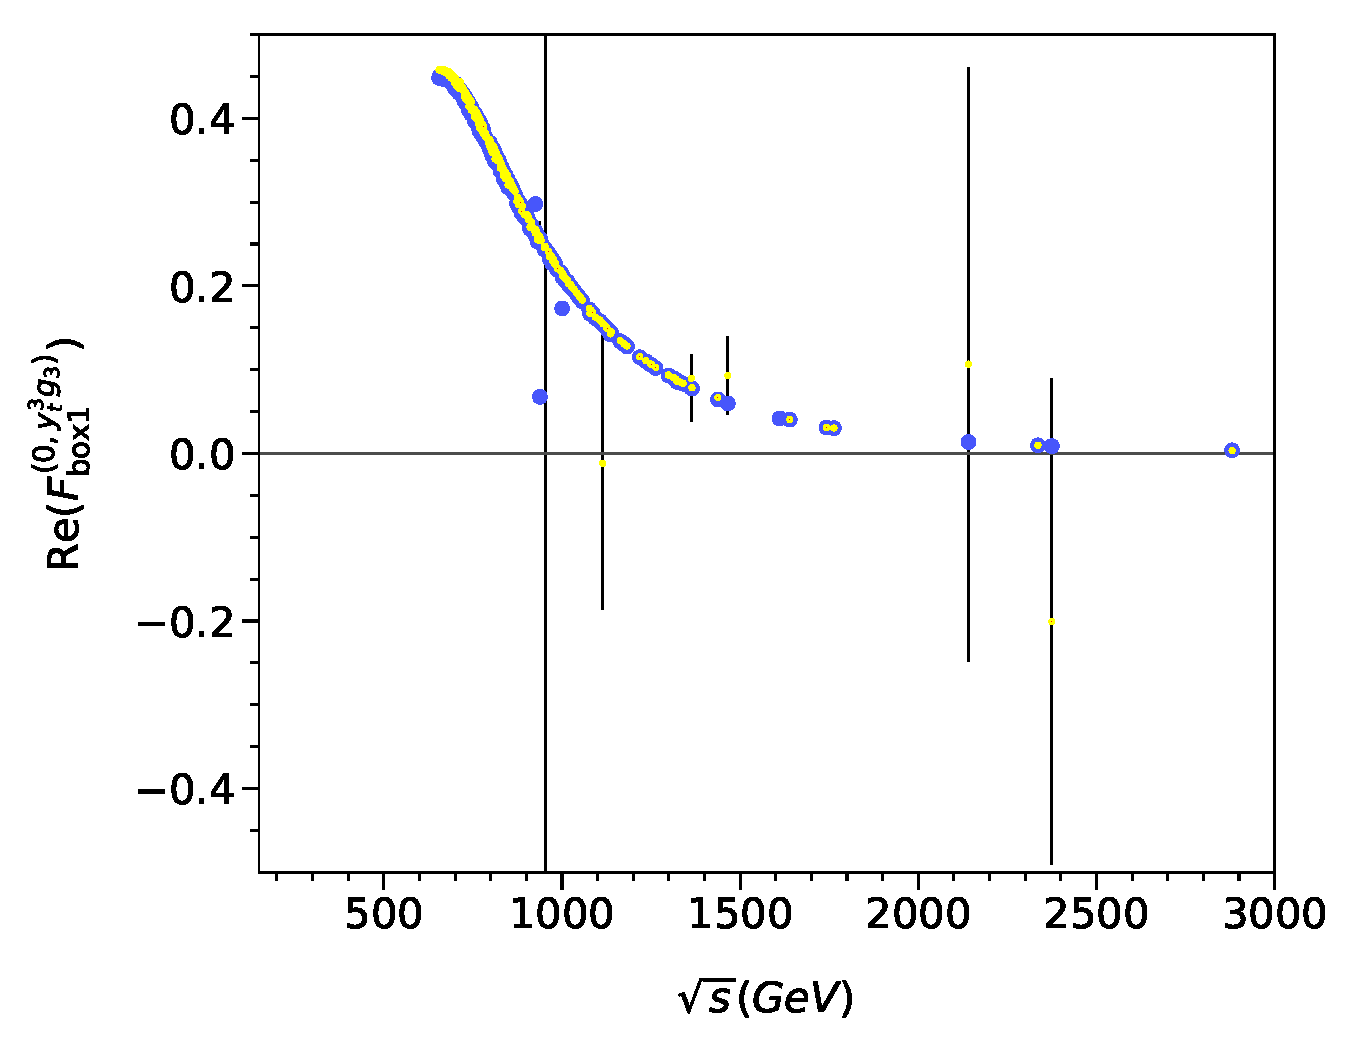
\includegraphics[width=0.48\textwidth]{NLO_EW_SM/EW_top-Higgs_self/Images/diff_to_SD_F1bare_ep0_t-plus_mhs2del3_yt3lam1_pTcut300_re_sqrts_FF}}}
	\\
    \subfloat[]{{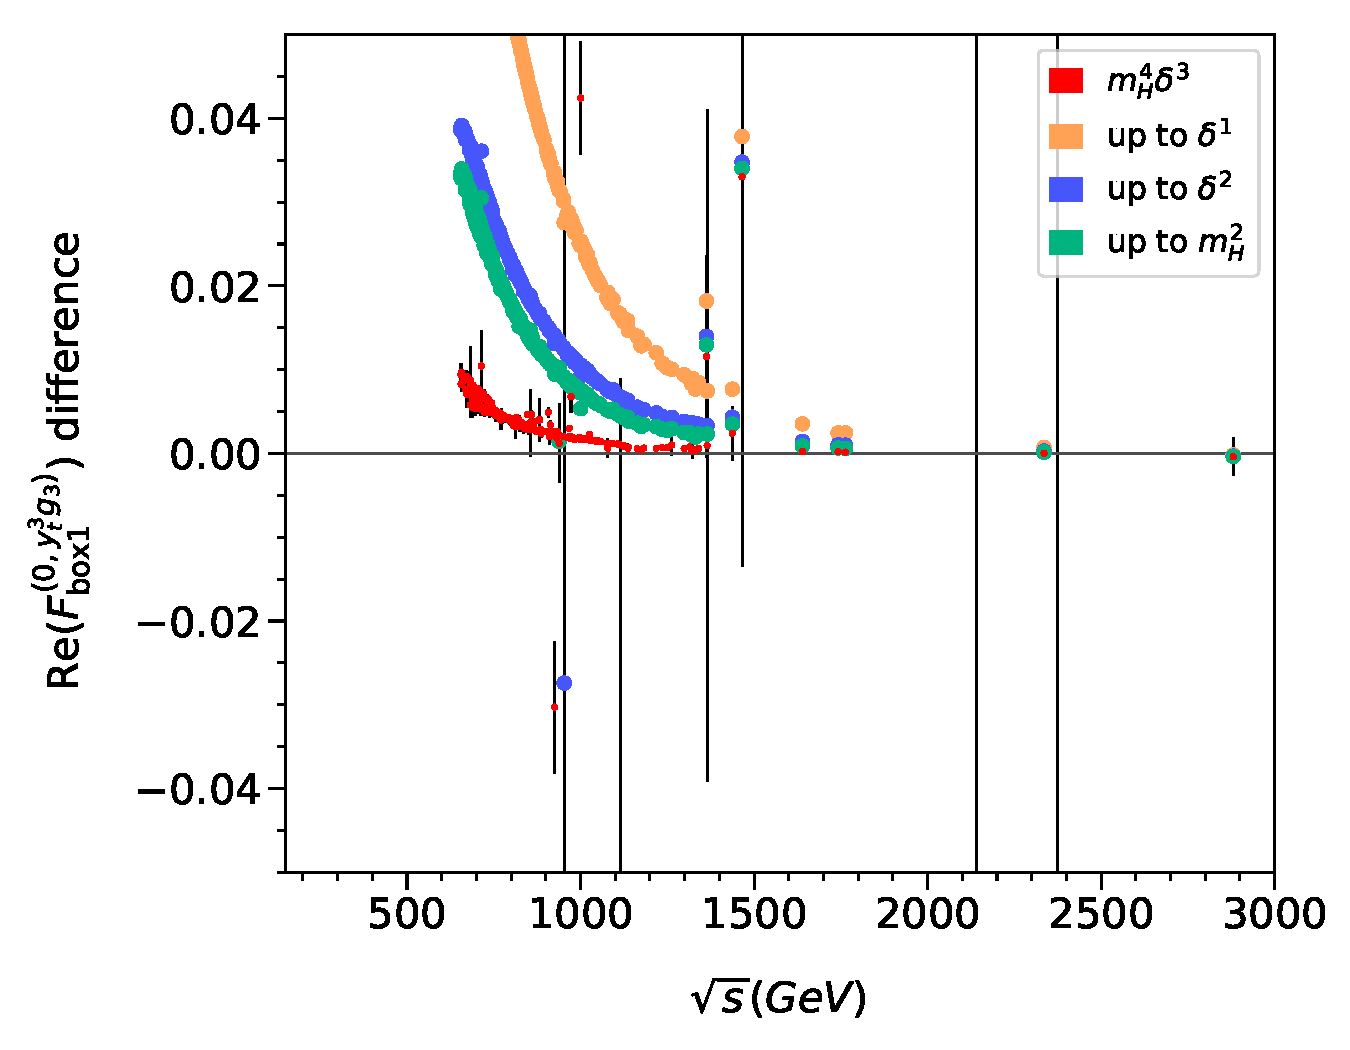
\includegraphics[width=0.48\textwidth]{NLO_EW_SM/EW_top-Higgs_self/Images/diff_to_SD_F1bare_ep0_t-plus_mhs2del3_yt3lam1_pTcut300_re_sqrts}}}
	\quad
    \subfloat[]{{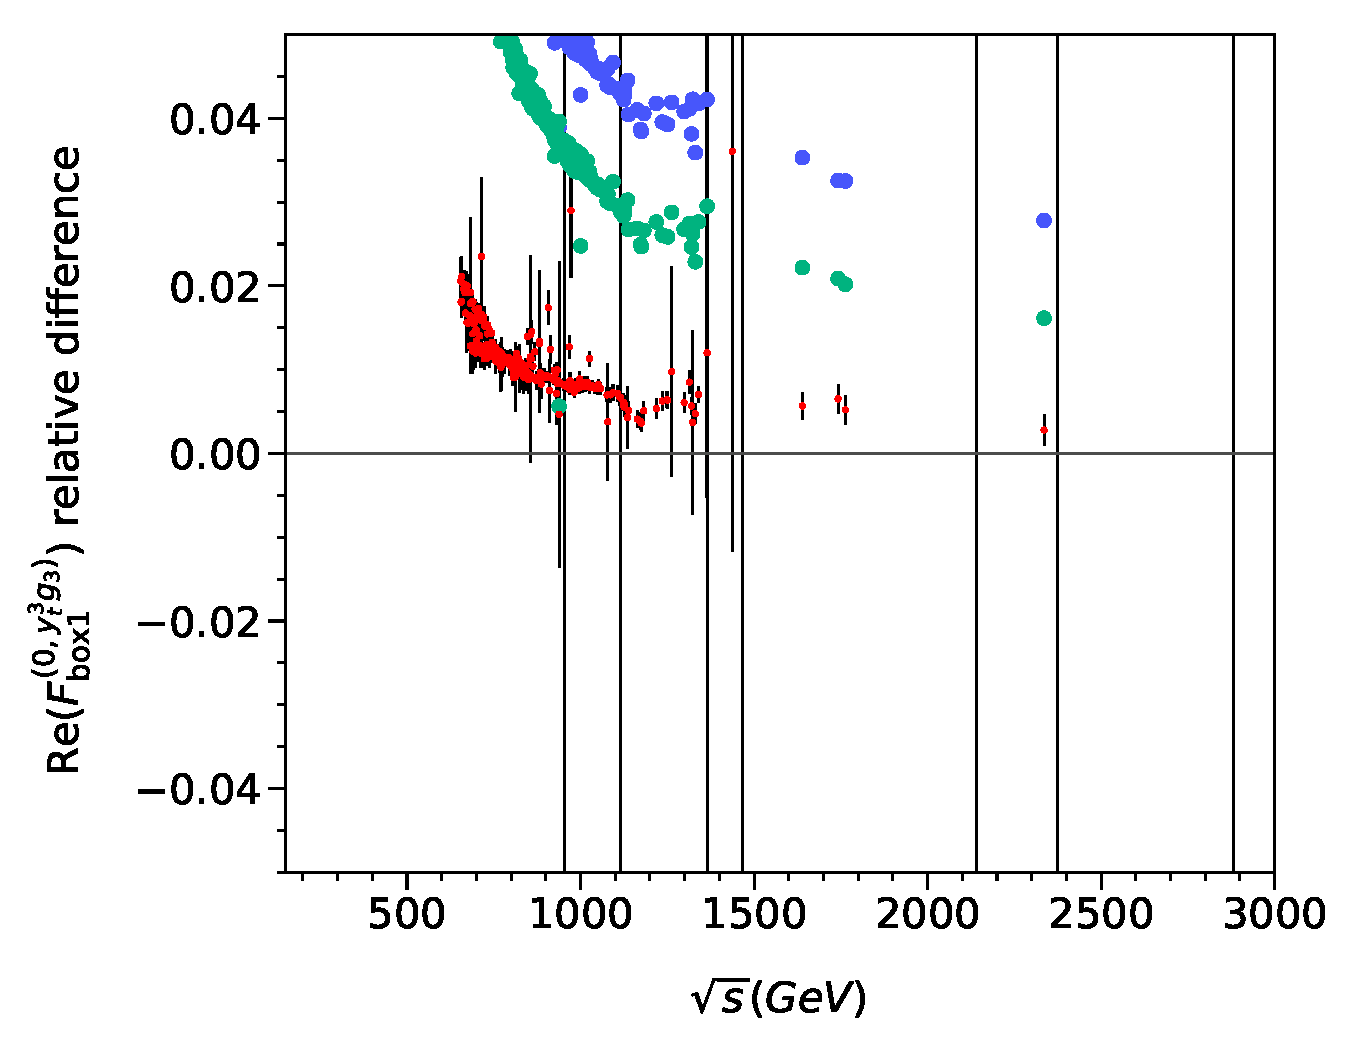
\includegraphics[width=0.48\textwidth]{NLO_EW_SM/EW_top-Higgs_self/Images/diff_to_SD_F1bare_ep0_t-plus_mhs2del3_yt3lam1_pTcut300_re_sqrts_rel}}}
	\caption{Real part of the form factor (a) from Feynman diagrams like those shown in Fig.~\ref{fig::diags}. (b) and (c) show the absolute and relative difference compared to Ref.~\cite{Heinrich:2024dnz}. Analytic results shown are from Ref.~\cite{Davies:2025wke}.}
    \label{fig::diff_to_SD_yt3lam1}
\end{figure}


\begin{figure}
\centering
    \subfloat[]{{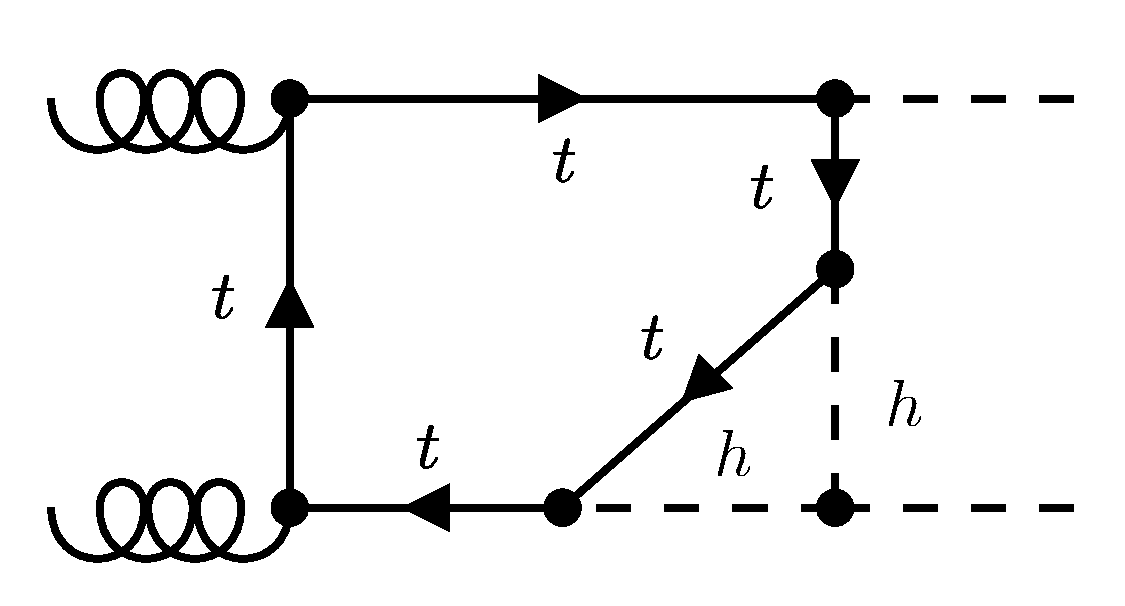
\includegraphics[width=0.3\textwidth]{NLO_EW_SM/EW_top-Higgs_self/Images/gghh_c_h.pdf}}}
	\quad
    \subfloat[]{{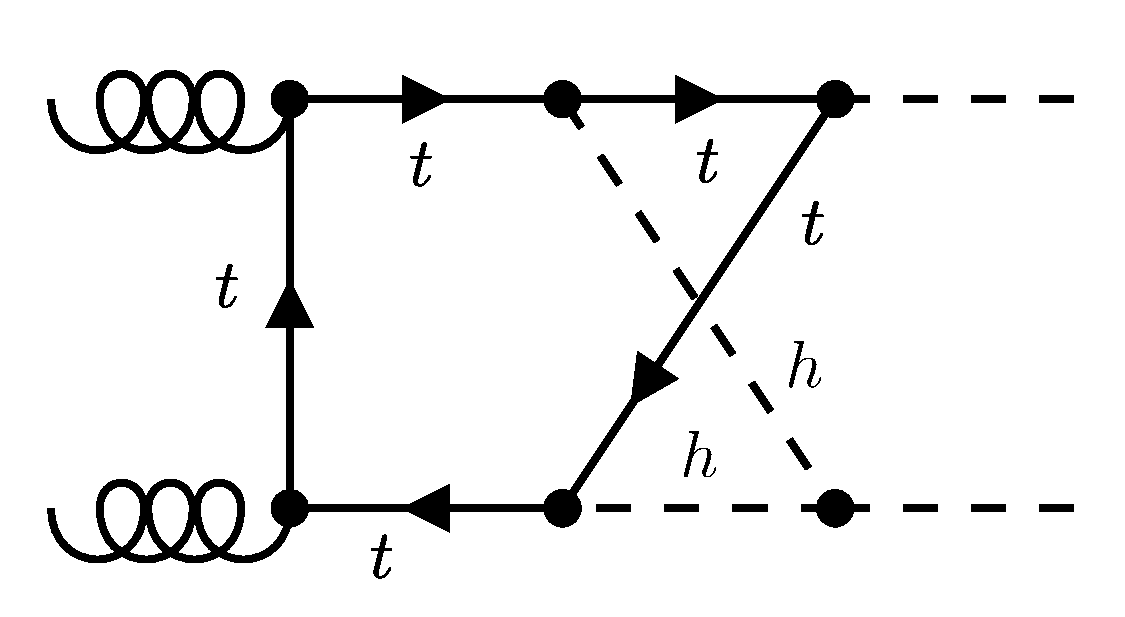
\includegraphics[width=0.3\textwidth]{NLO_EW_SM/EW_top-Higgs_self/Images/gghh_e_h.pdf}}}
	\caption{Sample Feynman diagrams. Solid, dashed and curly lines represent top quarks, Higgs bosons and gluons, respectively. Diagrams from Ref.~\cite{Davies:2025wke}.}
    \label{fig::diags}
\end{figure}


~

\noindent \textbf{Gudrun Heinrich, Stephen Jones, Matthias Kerner, Thomas Stone, Augustin Vestner~\cite{Heinrich:2024dnz}.}

\noindent In Ref.~\cite{Heinrich:2024dnz}, fully differential results for the Yukawa- and Higgs boson self-coupling-type electroweak corrections to Higgs boson pair production in gluon fusion are presented.
The results retain the full dependence on the mass of the top quark and the Higgs boson.
At the amplitude level, the results are further separated into the individual coupling structures, allowing for the bare amplitude to be computed with arbitrary top Yukawa coupling, trilinear Higgs boson self-coupling, and quartic Higgs boson self-coupling.

The precise class of corrections which are computed is defined via a Yukawa model with only an up-type quark (the top quark) and a scalar field (the Higgs boson). Example Feynman diagrams are shown in Fig.~\ref{fig:240704653_examplediags}.
This model selects a well-defined subset of diagrams which can be obtained from considering the SM in the unitary gauge and then setting $(g, g^\prime) \rightarrow (0,0)$, which removes the electroweak gauge bosons (and their associated ghost fields).
The electroweak input-parameter scheme $\left\{ M_Z=0, M_W=0, G_F\right\}$ + $\left\{m_t,m_h\right\}$ is used, where all masses are specified in the on-shell scheme.
Results are presented with the Higgs vev fixed in the $G_\mu$ scheme (with $M_Z=0$, $M_W=0$). However, the intermediate results are sufficiently general to allow another renormalization scheme to be adopted.
Tadpole contributions are treated within the Fleischer--Jegerlehner tadpole scheme (FJTS)~\cite{Fleischer:1980ub}.


\begin{figure}
\centering
    \subfloat[]{{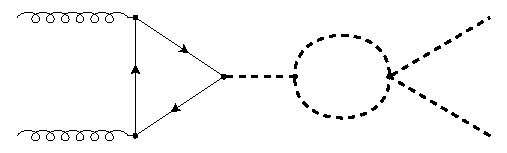
\includegraphics[width=0.3\textwidth]{NLO_EW_SM/EW_top-Higgs_self/Images/NLOtritpropHbubH}}}
	\qquad
    \subfloat[]{{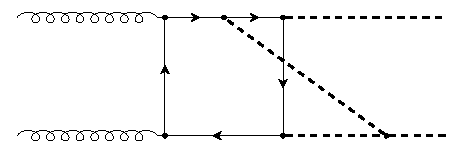
\includegraphics[width=0.3\textwidth]{NLO_EW_SM/EW_top-Higgs_self/Images/NLOboxHvertcorr}}}
	\qquad
    \subfloat[]{{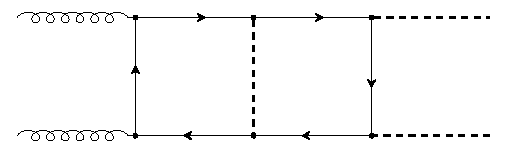
\includegraphics[width=0.3\textwidth]{NLO_EW_SM/EW_top-Higgs_self/Images/NLOboxtboxt}}}
		\caption{Example diagrams contributing to the different coupling structures into which the bare two-loop amplitude is separated. Diagrams from Ref.~\cite{Heinrich:2024dnz}.}
    \label{fig:240704653_examplediags}
\end{figure}


The calculation is performed by projecting the bare amplitude onto the two form factors described above in $D=4-2\epsilon$ dimensions.
The unreduced amplitude is obtained using two separate calculations based on either \texttt{alibrary}~\cite{alibrary}, a \texttt{Mathematica} and \texttt{Form}~\cite{Kuipers:2013pba} package for computing multi-loop amplitudes, or \texttt{Reduze 2}~\cite{vonManteuffel:2012np}, allowing for a detailed cross-check.
The form factors are then reduced fully symbolically, retaining the dependence on the Mandelstam invariants ($s$, $t$), the masses ($m_h$, $m_t$) and the space-time dimension $D$, to a basis of 494 finite master integrals using the public programs \texttt{Kira}~\cite{Klappert:2020nbg}, \texttt{Ratracer}~\cite{Magerya:2022hvj}, and \texttt{Firefly}~\cite{Klappert:2019emp,Klappert:2020aqs}.
The master integrals appearing in the reduced form factors are then evaluated numerically for each phase-space point using \texttt{pySecDec}~\cite{Borowka:2017idc,Borowka:2018goh,Heinrich:2021dbf,Heinrich:2023til}. The evaluation of the master integrals is additionally cross-checked at several physical points using \texttt{DiffExp}~\cite{Hidding:2020ytt,Moriello:2019yhu}.


\begin{figure}
\centering
    \subfloat[]{{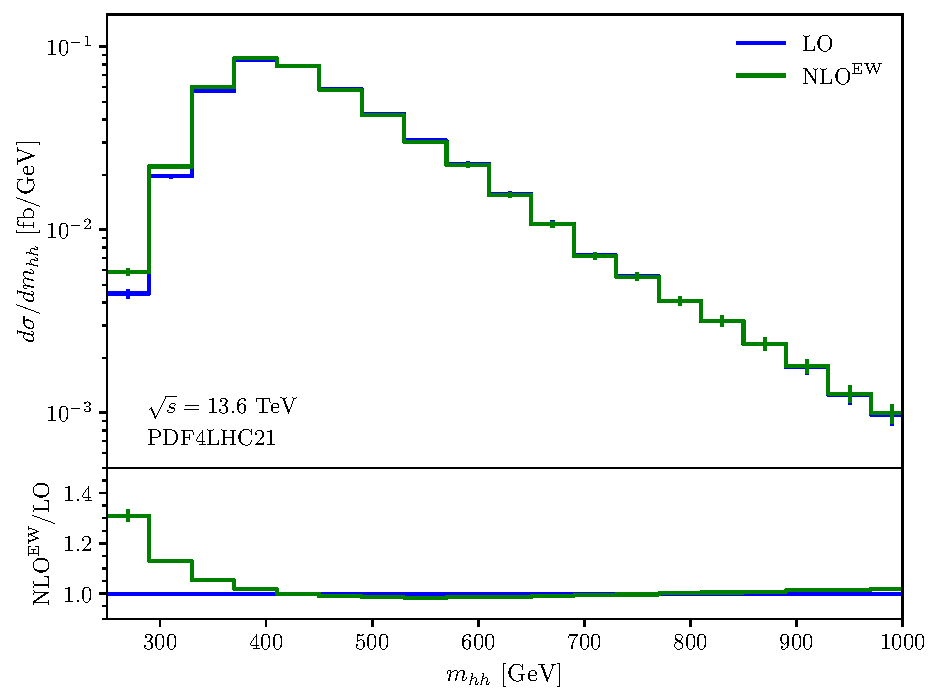
\includegraphics[width=0.48\textwidth]{NLO_EW_SM/EW_top-Higgs_self/Images/mhh_full_h.pdf}}}
	\quad
    \subfloat[]{{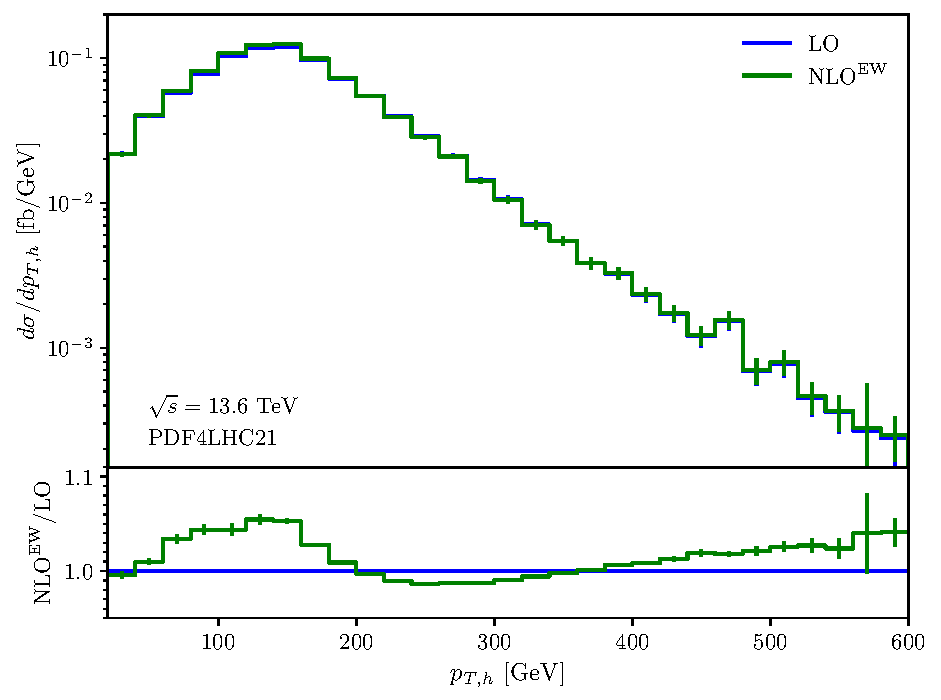
\includegraphics[width=0.48\textwidth]{NLO_EW_SM/EW_top-Higgs_self/Images/pth_full_h.pdf}}}
    \caption{Invariant mass (a) and transverse momentum (b) distributions for Higgs boson pair production at LO and $\mathrm{NLO}^\mathrm{EW}$ including only the Yukawa and Higgs boson self-coupling-type corrections. Results shown are from Ref.~\cite{Heinrich:2024dnz}.}
    \label{fig:240704653_dists}
\end{figure}


In Fig.~\ref{fig:240704653_dists}, results for the Higgs boson pair invariant mass and $p_{T,H}$~distribution are shown.
The results presented here are obtained using the \texttt{PDF4LHC21\_40}~\cite{PDF4LHCWorkingGroup:2022cjn} parton distribution functions interfaced via \texttt{LHAPDF}~\cite{Buckley:2014ana} and setting the factorization and renormalization scale to $\mu_r = \mu_f = m_{hh}/2$. The masses of the Higgs boson and top quark are set to $m_h = 125~\mathrm{GeV}$, $m_t = \sqrt{23/12}\,m_h = 173.055$ GeV, respectively, and $G_F = 1.1663787 \cdot 10^{-5}\,\textup{GeV}^{-2}$, corresponding to $v=246.22~\mathrm{GeV}$.
For the subset of the electroweak correction considered, very large shape distortions (around $30\%$ for the binning selected) are observed close to threshold for the invariant mass distribution, with much smaller corrections above $400\,\textup{GeV}$ (up to $1\,\textup{TeV}$).
The corrections in the $p_{T,H}$ distribution are less localized, with distortions of up to $5\%$ present across the spectrum.
Overall, the top Yukawa and Higgs boson self-coupling corrections amount to a $1\%$ enhancement of the total cross section.

An important observation concerns the renormalizability of models in which the top Yukawa coupling, the trilinear Higgs boson self-coupling, and the quartic Higgs boson self-coupling are varied from their SM values.
In particular, it is observed that the $1/\epsilon$ pole structure of the vev counterterm obtained by demanding the finiteness of the Yukawa or Higgs boson self-coupling vertices differs unless they are each set to their SM value.
This implies that the $\kappa$-framework used to extract the trilinear Higgs boson self-coupling modifier, $\kappa_\lambda \equiv \lambda_{hhh}/\lambda_{hhh}^{\rm SM}$, cannot directly be used when including the electroweak corrections to this process.
Furthermore, even though the quartic Higgs boson self-coupling first enters at $\mathrm{NLO}_\mathrm{EW}$, the subset of diagrams in which it appears is divergent prior to UV renormalization, implying that the $\kappa_4$ coupling also cannot naively be varied.
